% \section{Control Function (CF) Estimation of CM Effects}
% \label{sec:controlfun}
% This paper only considers a modern two-stage approach to selection models --- also known as a control function approach.
% Indeed, the conventional approach to estimating CM effects already uses a two-stage estimation procedure to estimate the first and second-stages.
% It is a simple, and intuition addition to include a two-stage control function adjustment to CM estimation.
% 
% Go through the steps of a Heckman selection model,  and the corresponding SEs + reference $\sqrt{n}$-consistency.
% Note Nancy Heckamn (1986) gives $\sqrt{n}$-consistency of splines.
% The two-stage semi-parametric procedure of Robinson (1988) is not appropriate, as we want the $\lambda_1(.)$ function, too.

\subsection{Simulation Evidence}
The following simulation gives an example to show how this method works in practice.
Suppose data observed to the researcher $Z_i, D_i, Y_i, \vec X_i$ are drawn from the following data generating processes, for $i = 1, \hdots, N$.
\begin{align*}
    Z_i \sim \text{Binom}\left(0.5 \right),
    \;\; \vec X_i^- \sim N(4, 1),
    \;\; \vec X_i^{\text{IV}} \sim \text{Binom}\left( 0.5 \right), \\
    \left( U_{0,i}, U_{1,i} \right) \sim
    \text{BivariateNormal}\left( 0, 0, \sigma_0, \sigma_1, \rho \right),
    \;\; U_{C,i} \sim N(0, 0.5).
\end{align*}
$N = 10,000$ allows the large sample properties of the approach to operate; indeed, smaller sample sizes may not.

Suppose each $i$ chooses to take mediator $D_i$ by a Roy model, with following mean definitions for each $z', d' = 0, 1$.
\begin{align*}
    D_i(z') = \indicator{Y_i(z', 1) - Y_i(z', 0) \geq C_i},  \\
    \mu_{d'}\left(z' ; \vec X_i \right) = \vec X_i^- + \left( z' + d' + z' d' \right),
    \;\; \mu_{C}\left(z' ; \vec X_i \right) = 3z' + \vec X_i^- - \vec X_i^{\text{IV}}.
\end{align*}
Following \autoref{sec:applied}, these data have the following first and second-stage equations:
\begin{align*}
    D_i &= \indicator{-3Z_i - \vec X_i^{\text{IV}} + \vec X_i^-
        \geq U_{C,i} - \Big( U_{1,i} - U_{0,i} \Big)},  \\
    Y_i &= Z_i + D_i + Z_i D_i + \vec X_i^-
        + \left( 1 - D_i \right) U_{0,i} + D_i U_{1,i}.
\end{align*}
$Z_i$ has an effect on outcome $Y_i$, and it operates partially through mediator $D_i$.
Outcome mean $\mu_{D_i}(Z_i;.)$ contains an interaction term, $Z_i D_i$, so while both $Z_i$ and $D_i$ have constant partial effects, the ATE depends on how many $i$ choose to take the mediator.
In this simulation $\Prob{D_i = 1} = 0.437$, and $65.29\%$ of the sample are mediator compliers (where $D_i(1)=1$ and $D_i(0) = 0$).
This gives an ATE ($Z\to Y$) value of 2.58, ADE 1.44, and AIE 1.13, respectively.\footnote{
    Note that ATE $=$ ADE $+$ AIE in this setting.
    $\Prob{Z_i=1} = 0.5$ ensures this equality, but it is not guaranteed in general.
}

After $Z_i$ is assigned, $i$ chooses to take mediator $D_i$ by considering the costs and benefits --- which vary based on $Z_i$, demographic controls $\vec X_i$, and the (non-degenerate) unobserved error terms $U_{i,0}, U_{1,i}$.
As a result, sequential ignorability does not hold; the mediator is not conditionally ignorable.
Thus, a standard OLS (selection-on-observables) approach to CM does not give an estimate for how much of the $Z \to Y$ ATE goes through mediator $D$.
Instead, the OLS approach gives biased inference.
The bias in OLS estimates comes from the unobserved error terms being related.

The CF estimator here uses the inverse Mills ratio as the CFs (i.e., a Heckman selection model); in-progress work develops a constrained semi-parametric approach to model $\lambda_0$ (and thus $\lambda_1$) to avoid distributional assumptions.
\autoref{fig:cm-heckit-dist} shows the distribution of simulated point estimates in this simulation, showing OLS against the CF approach.
The OLS approach implicitly assumes that the mediator is ignorable (when it is not), so its point estimates under and over-estimate the true ADE and AIE, respectively.
The distance between the OLS estimates and the true values are the underlying bias terms derived in \autoref{thm:selection-bias}.
In this data generating process, the OLS confidence interval do not overlap the true values for any standard level of significance.
The CF approach exhibits bias, though the 95\% confidence intervals cover the truth.

\begin{figure}[h!]
    \caption{Point Estimates of CM Effects, OLS versus CF, varying $\rho$ values with $\sigma_0 = 1, \sigma_1 = 2$ fixed.}
    \begin{subfigure}[c]{0.475\textwidth}
        \centering
        \caption{ADE.}
        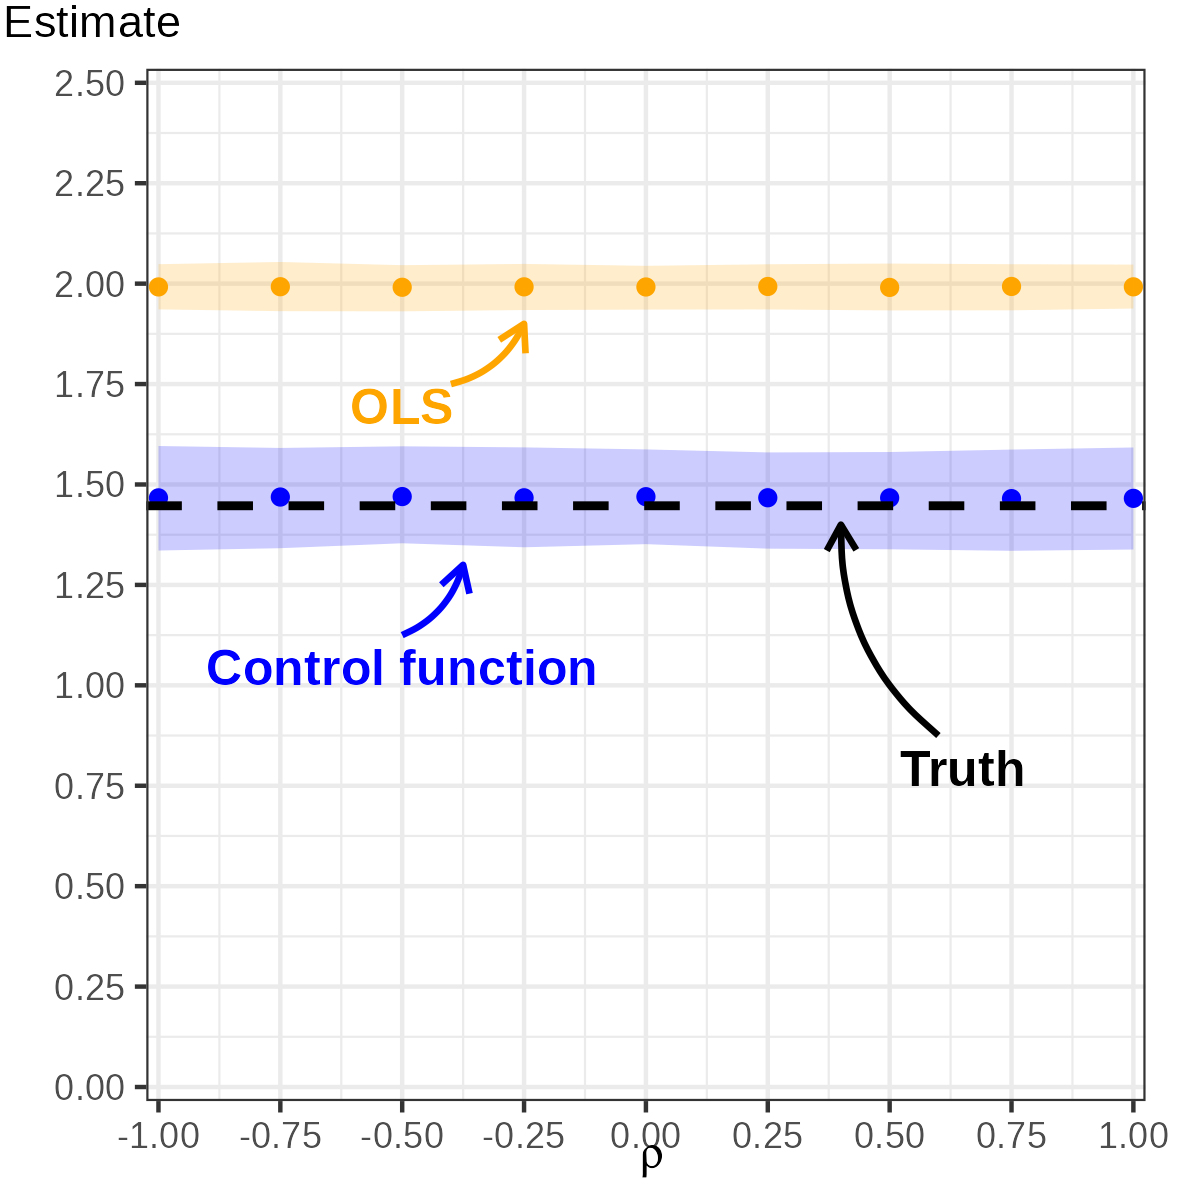
\includegraphics[width=\textwidth]{
            ../programs/simulations/sim-output/rho-directeffect-bias.png}
    \end{subfigure}
    \begin{subfigure}[c]{0.475\textwidth}
        \centering
        \caption{AIE.}
        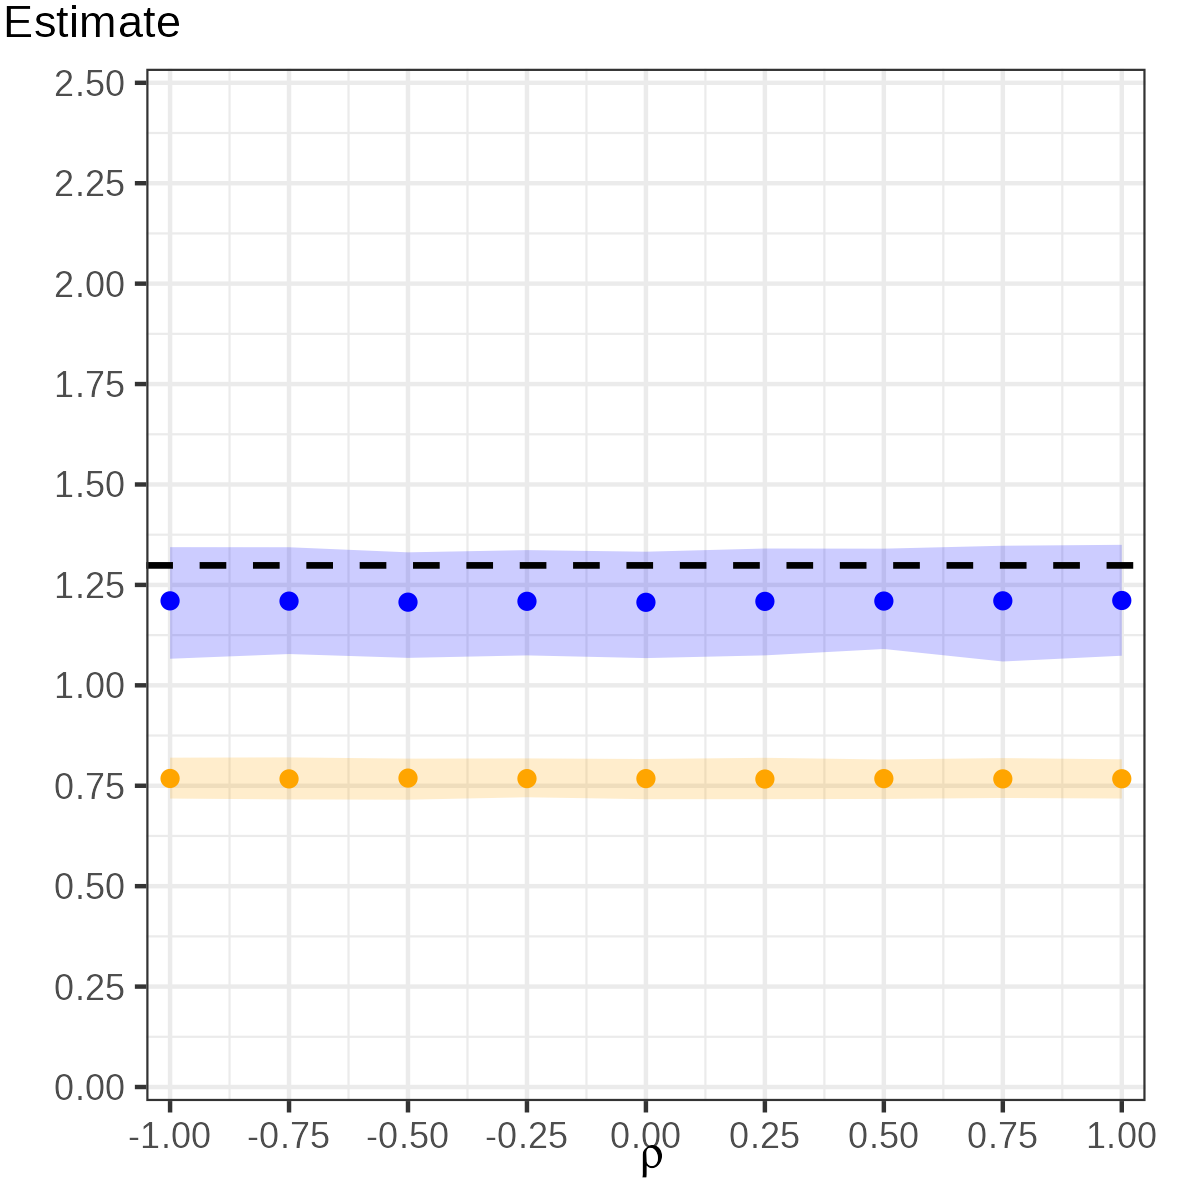
\includegraphics[width=\textwidth]{
            ../programs/simulations/sim-output/rho-indirecteffect-bias.png}
    \end{subfigure}
    \label{fig:rho-bias}
    \justify
    \footnotesize    
    \textbf{Note:}
    These figures show the OLS and CF point estimates of the ADE and AIE, for $N = 10,000$ sample size.
    The black dashed line is the true value, points are points estimates from data simulated with a given $\rho$ value and $\sigma_0 = 1, \sigma_1 = 2$, and shaded regions are the 95\% confidence intervals from 1,000 bootstraps each.
    Orange represents OLS estimates, blue the CF approach.
    The true AIE values vary with $\rho$, because $D_i(Z_i)$ compliers have higher average values of $U_{1,i} - U_{0,i}$ with greater $\rho$ values.
\end{figure}

The error terms determine the bias in OLS estimates of the ADE and AIE, so the bias varies for different values of the error-term parameters $\rho \in [-1, 1]$ and $\sigma_0, \sigma_1 \geq 0$.\footnote{
    Indeed, this setting has error terms following a bivariate normal distribution, so the canonical \cite{heckman1974shadow} selection model would produce the most efficient estimates by maximum likelihood.
    The CF approach avoids this assumption, and bias from breaking it, by relying on an instrument.
}
\autoref{fig:rho-bias} shows CF estimates against estimates calculated by standard OLS, showing 95\% confidence intervals calculated from 1,000 bootstraps.
The point estimates of the CF do not exactly equal the true values, as they are estimates from one simulation (not averages across many simulations, as in \autoref{fig:cm-heckit-dist}).
The CF approach improves on OLS estimates by correcting for bias, with confidence regions overlapping the true values.\footnote{
    The code behind this simulation estimates the first-stage with an interacted OLS specification.
    The second-stage is an OLS specification, including the CFs.
    The in-progress semi-parametric approach uses a spline specification for $\lambda_1$ in the $D_i = 1$ sample, and $\lambda_0$ in the $D_i = 0$ sample, composing a moment restricted estimate of $\lambda_1$ from these. 
}$^,$\footnote{
    In the appendix, \autoref{fig:sigma-bias} shows the same simulation while varying $\sigma_1$, with fixed $\sigma_0 = 1, \rho = 0.5$.
    The conclusion is the same as for varying the correlation coefficient, $\rho$, in \autoref{fig:rho-bias}.
}
This correction did not come for free: the standard errors are significantly greater in a CF approach than OLS.
Standard errors on the AIE are larger than those for the ADE, because the AIE estimates are first-stage times second-stage estimates, so standard errors account for uncertainty in both estimates multiplied.
%(i.e., the same reasons instrumental variables estimates are less efficient than ideal OLS estimates). 
In this manner, this simulation shows the pros and cons of using the CF approach to estimating CM effects in practice.
